\chapter{Сущность решения задачи}

Описанные выше технические требования нашли своё отражение в сущности решения задачи предоставления удобного сервиса для создания, обучения и общения с цифровыми двойниками. Решение было дифференцированно на несколько независимых сущностей, каждая из которых была материализованна в соответствующие компоненты системы.

\section{Компоненты решения}
\subsection{Веб интерфейс}
Веб интерфейс отвечает за взаимодействие с пользователем и именно с его помощью пользователь будет посылать запросы внутрь системы. Так же этот компонент системы будет отвечать за то, чтобы потребитель получил результат работы сервиса в удобном и интуитивно понятном формате.

\subsection{Бекэнд}
Бекэнд необходим для запуска запрошенных процедур со стороны пользователя через веб интерфейс. Помимо этого компонент занимается оркестрацией всего сервиса, первичной предобработкой данных, полученных от пользователя и возврата промежуточных и итоговых результатов работы сервиса.

\subsection{Реляционная база данных}
Реляционная база данных предоставляет среду для хранения метаданных пользователя и аватаров, состояния системы, а так же быстрого поиска, вставки и модификации этих данных. Так же для корректной работы системы необходимо, чтобы данные оставались валидными в условиях конкурентного исполнения, что так же является зоной ответственности этого компонента.

\subsection{ML сервис}
ML сервис занимается непосредственным обучением моделей и генерацией данных для создания ответа и его озвучки на запрос пользователя с помощью ранее обученных моделей. Причем после обучения модели для конкретного цифрового двойника этот сервис должен обеспечить возможность быстрого взаимодействия без повторного обучения модели при последующем обращении. Поэтому данный компонент контролирует сохранение и выгрузку весов моделей, полученных в результате процедуры обучения на пользовательских данных.

\subsection{Брокер сообщений}
Брокер сообщений является сердцем всей системы, так как он предоставляет отказоустойчивую и отзывчивую среду для организации межкомпонентного взаимодействия системы.

\subsection{S3 хранилище}
S3 хранилище обеспечивает хранение, обновление и удаление больших по объему данных, которые не укладываются или их хранение является неэффективным в контексте реляционных баз данных.

\section{Алгоритм взаимодействия}

\subsection{Процедуры регистрации и аутентификации пользователя}
Нельзя забывать о том, что мы работаем с данными пользователя, значит, нельзя забывать и о конфиденциальности. Поэтому помимо непосредственного решения поставленной задачи необходимо позаботиться о защищенности данных. Самый простой и надежный способ сделать это - добавить функционал аутентификации пользователей. Таким образом сервис сможет гарантировать, что доступ к данным будет оставаться только у владельца соответствующей учетной записи. На диаграмме процесса регистрации и аутентификации (рис. \ref{fig:uf-log-or-reg}) описаны шаги, которые пользователь проходит от момента перехода на веб страницу сервиса до перехода в личный кабинет, который предоставляет интерфейс по управлению аватарами.

\begin{figure}[h!]
     \centering
     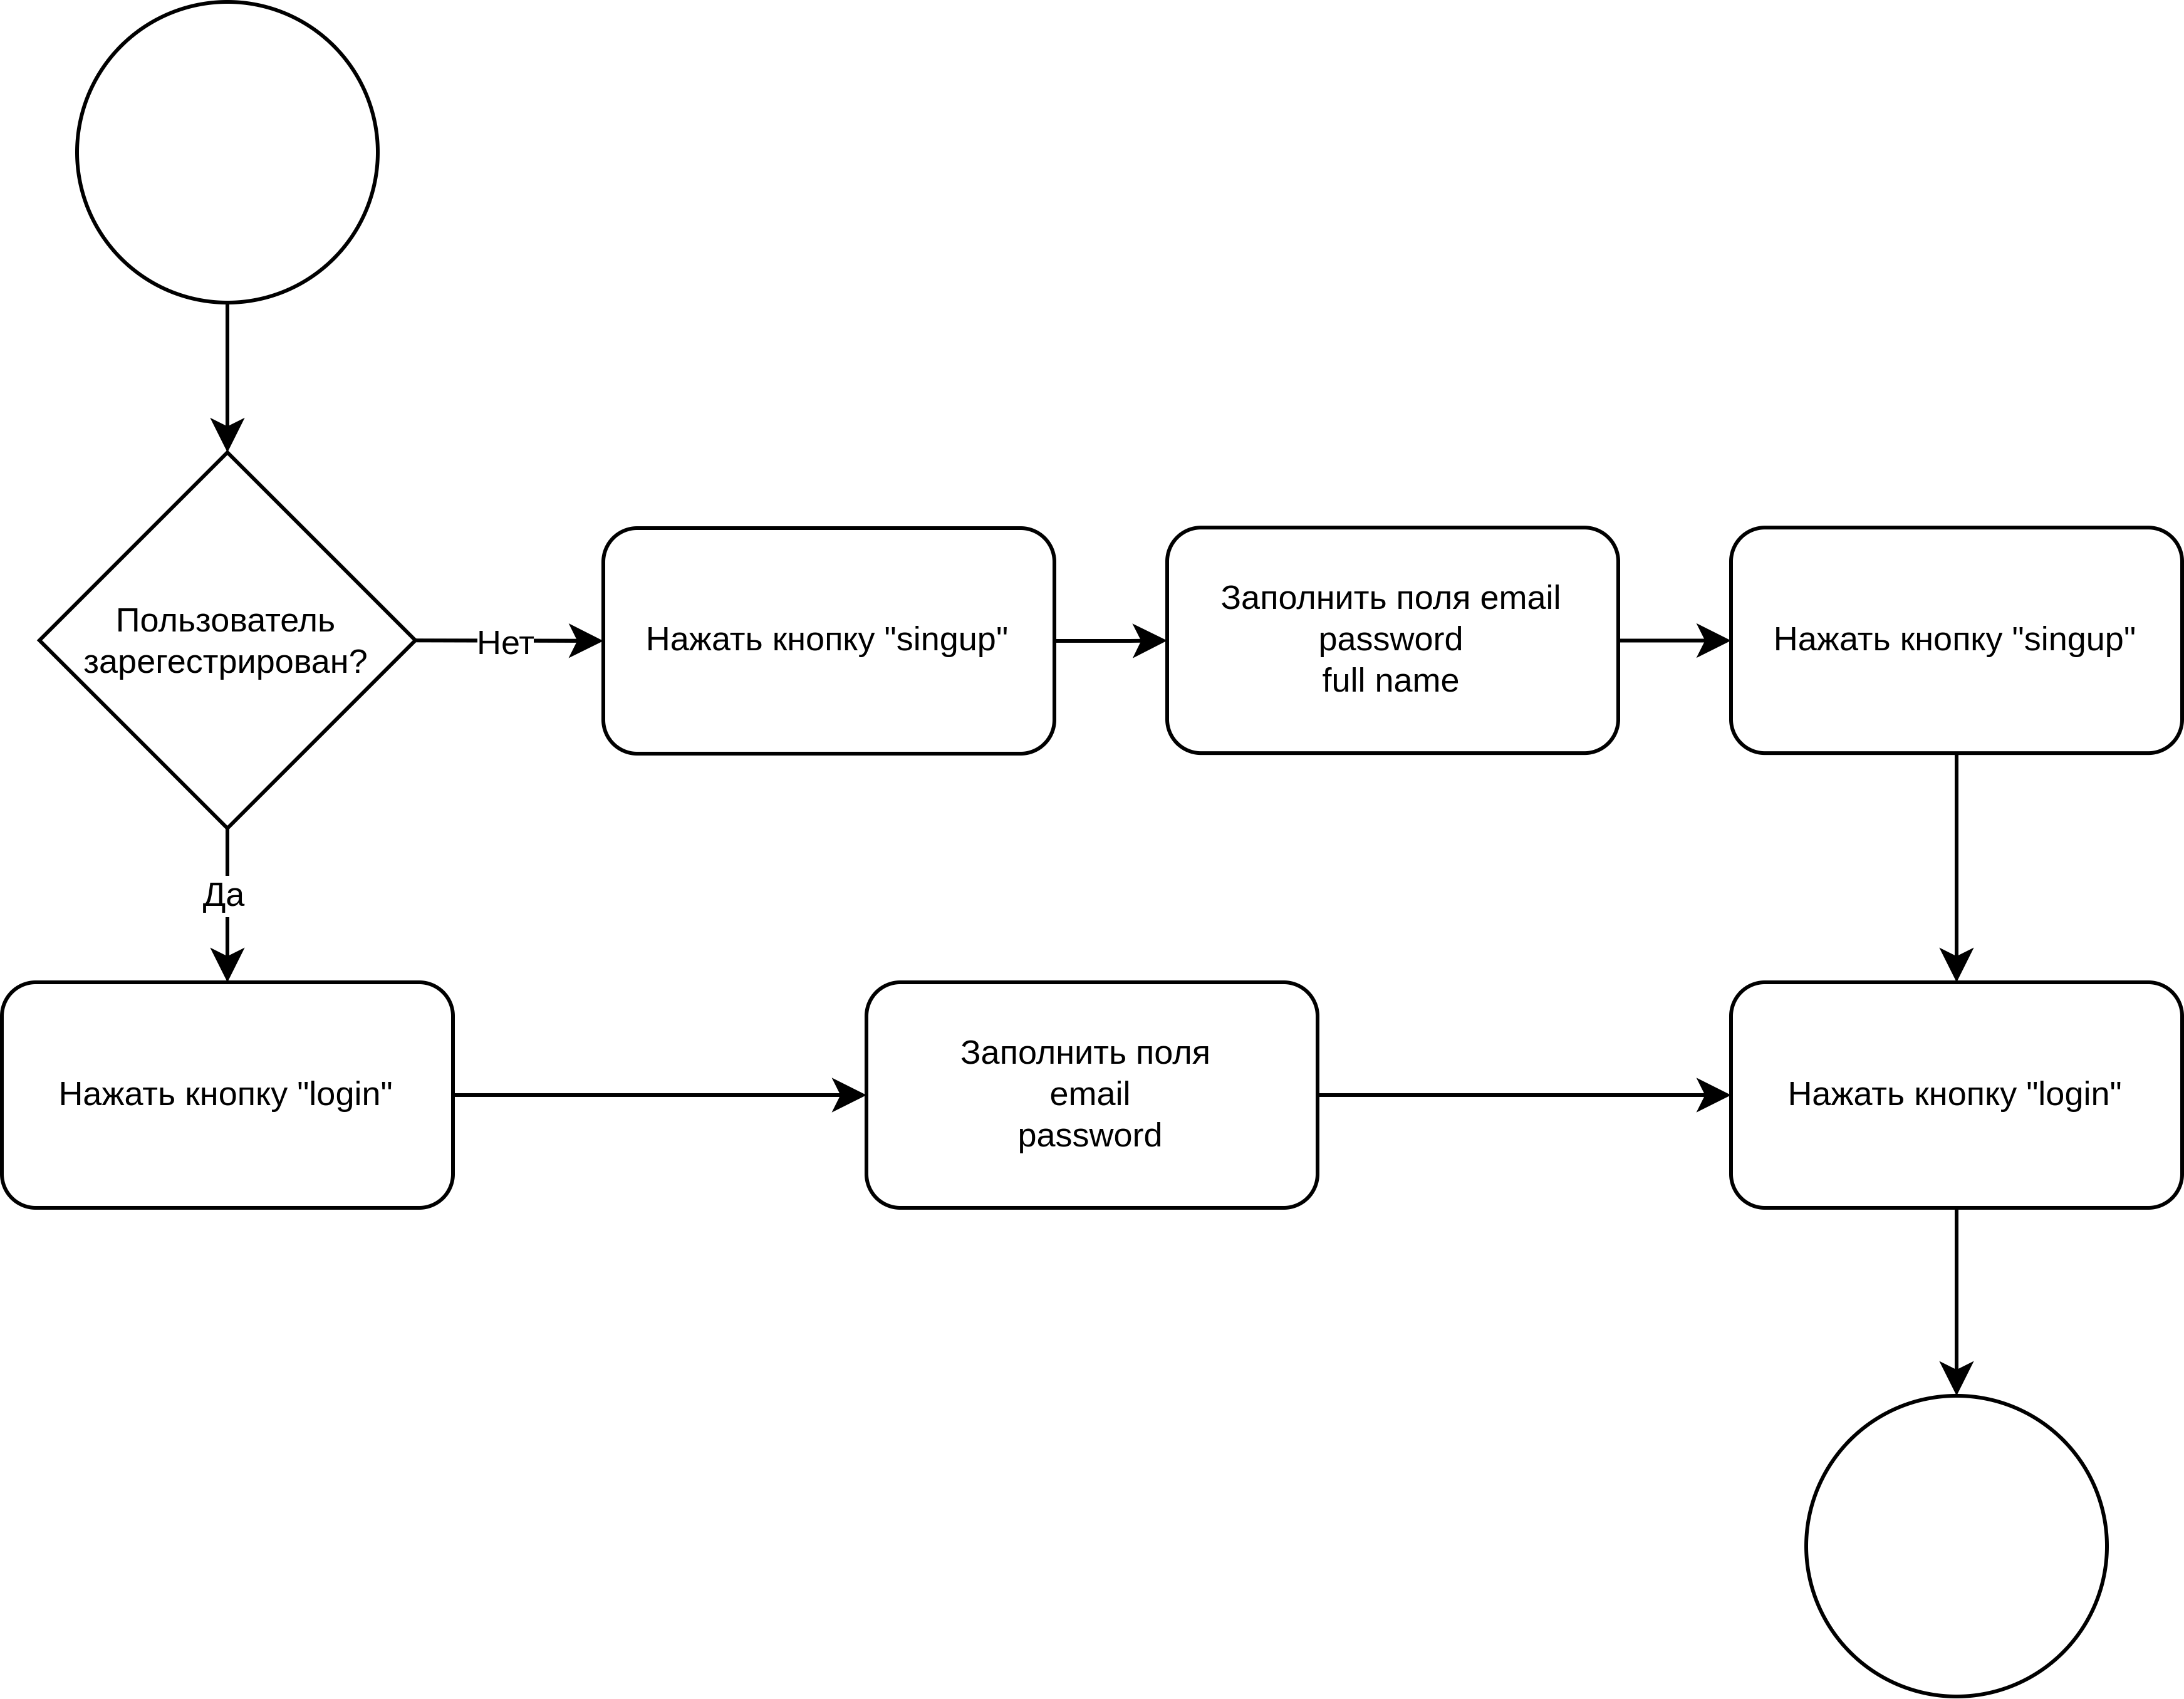
\includegraphics[width=1.0\linewidth]{images/UF-login-or-reg.png}
     \caption{User flow диаграмма процесса регистрации или авторизации}
     \label{fig:uf-log-or-reg}
\end{figure}

\subsection{Процедура обучения}
Решение имеет микросервисную архитектуру. Это значит, что весь сервис разбит на ряд независимых с точки зрения физического расположения компонент, а взаимодействие между ними происходит через сеть с помощью брокера сообщений. На диаграмме обучения аватара (рис. \ref{fig:uml-train}) представлены основные сообщения и события, которые происходят в системе для получения желаемого результата. Так же на user flow диаграмме (рис. \ref{fig:uf-train}) показано какие именно действия производит пользователь для обучения существующего или создания и обучения нового аватара.

 \begin{figure}[h!]
     \centering
     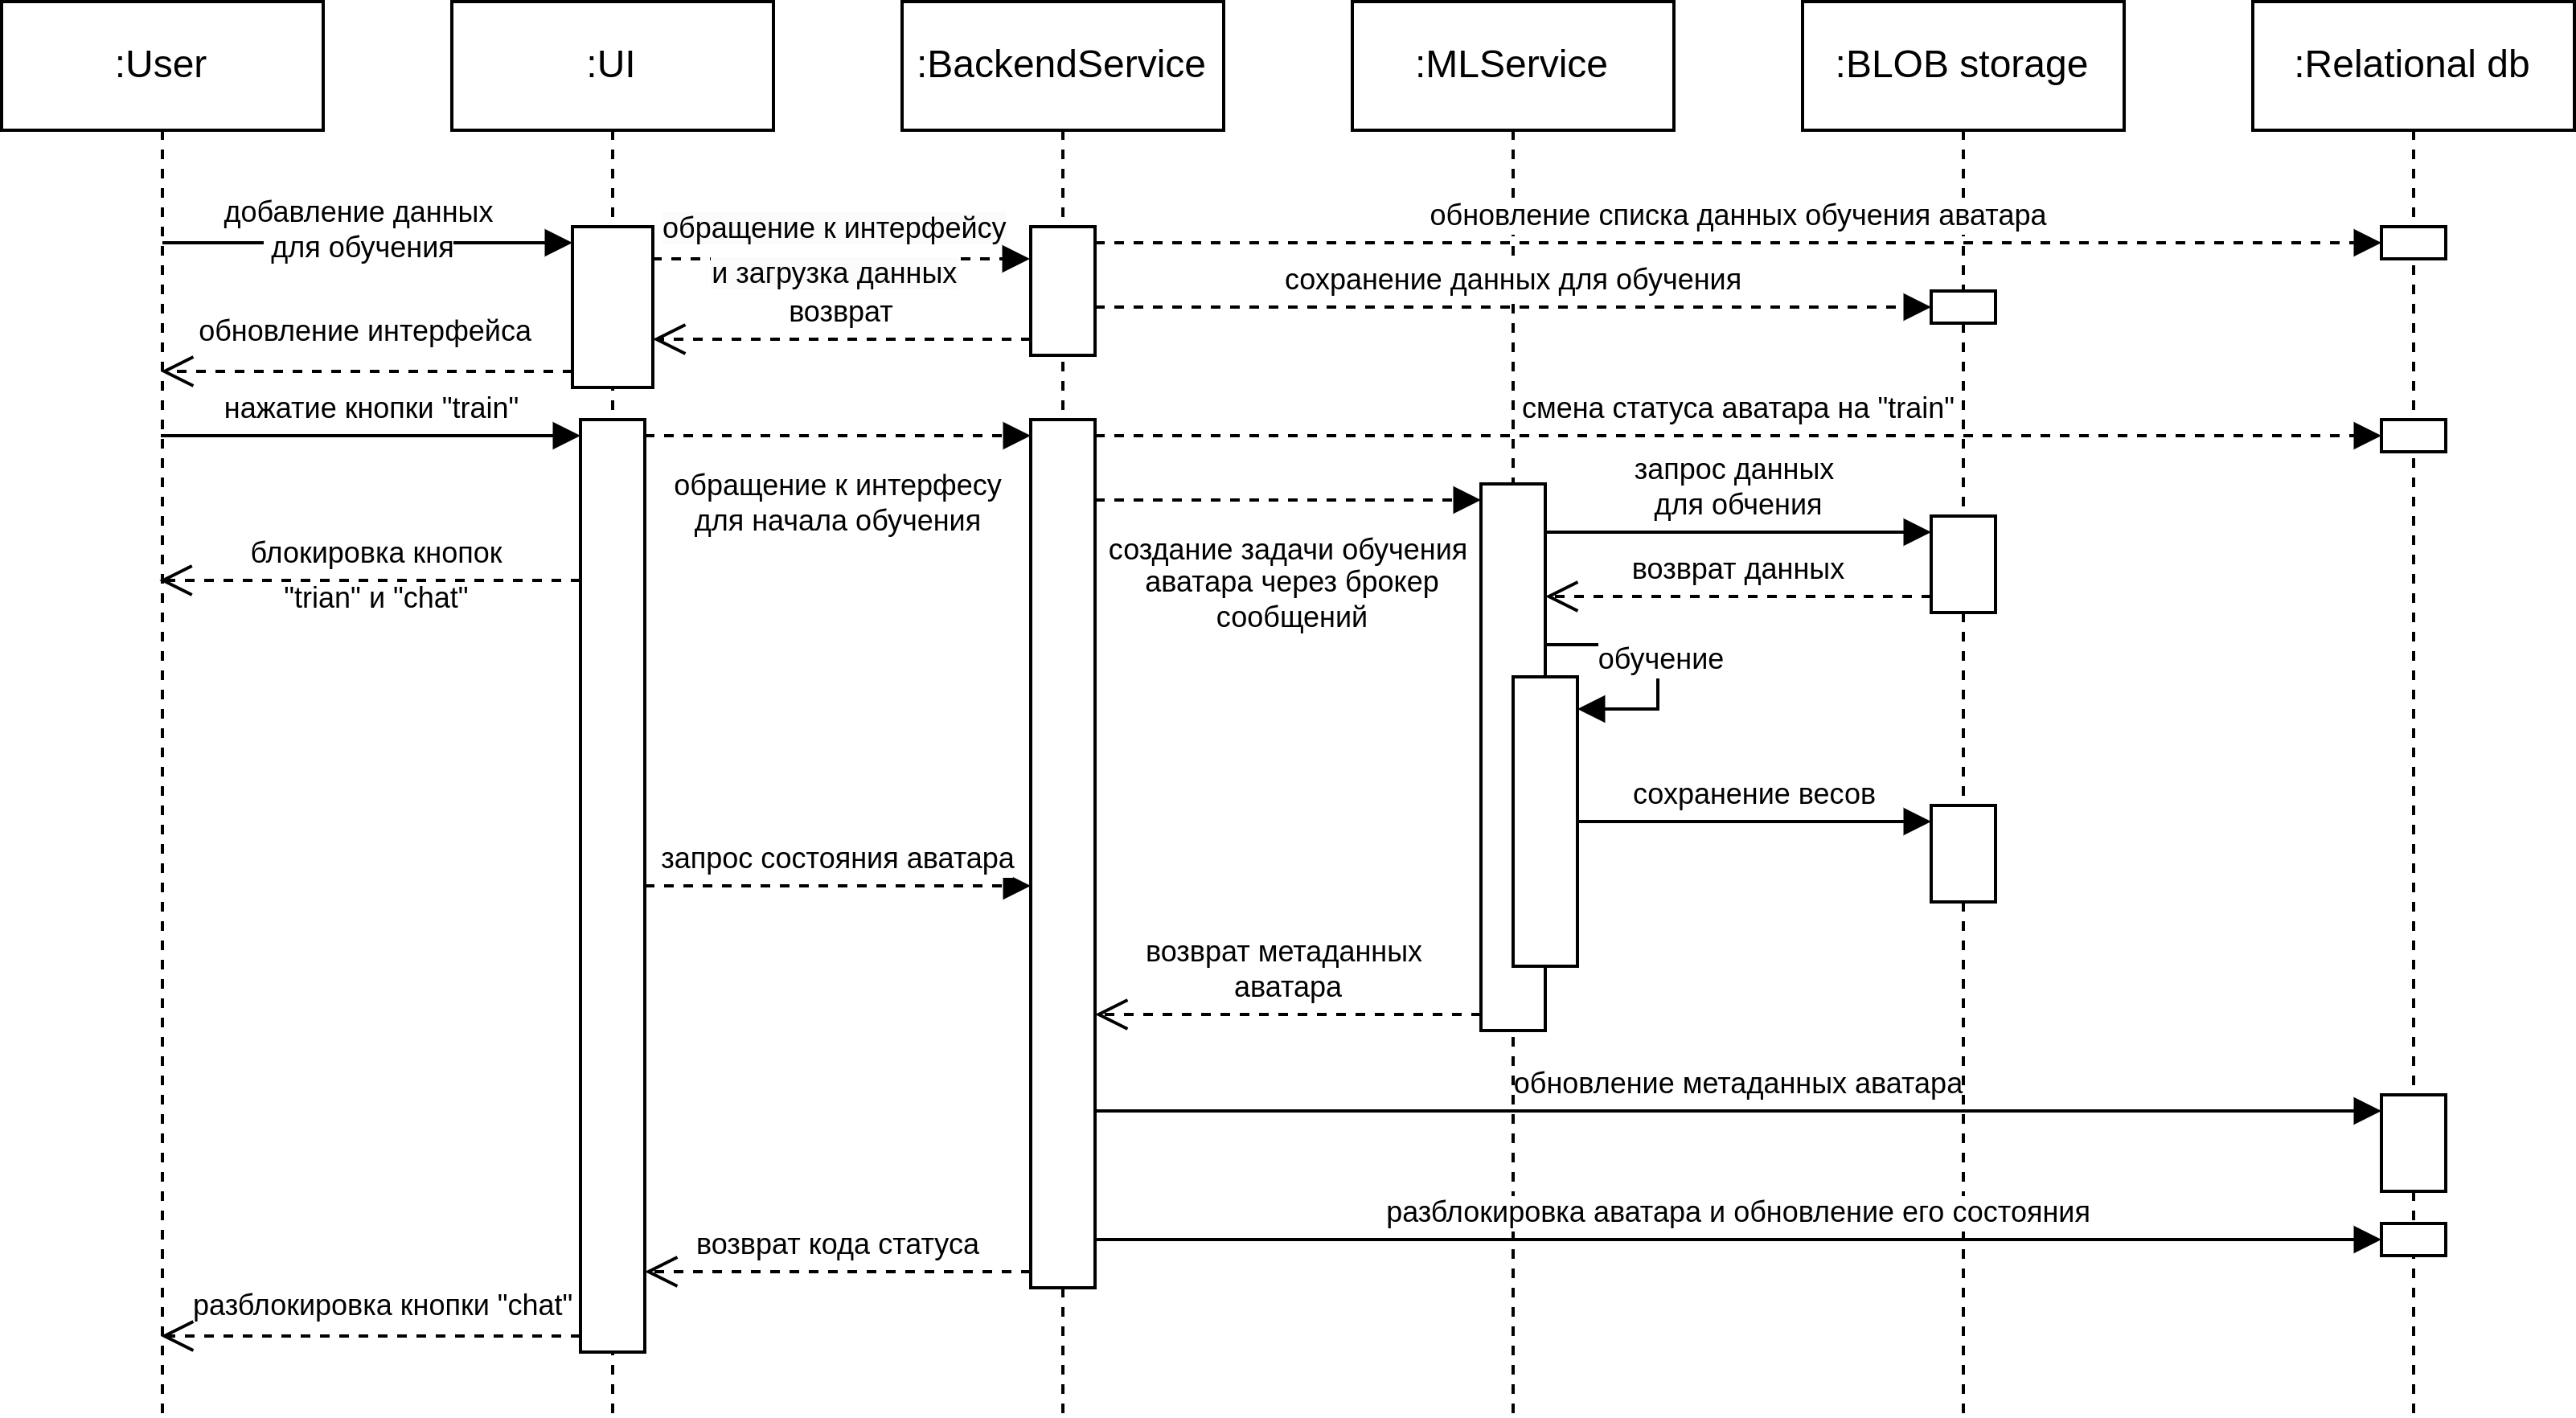
\includegraphics[width=1.0\linewidth]{images/uml-train-rus.png}
     \caption{UML-диаграмма процесса обучения}
     \label{fig:uml-train}
 \end{figure}
 \begin{figure}[h!]
    \centering
    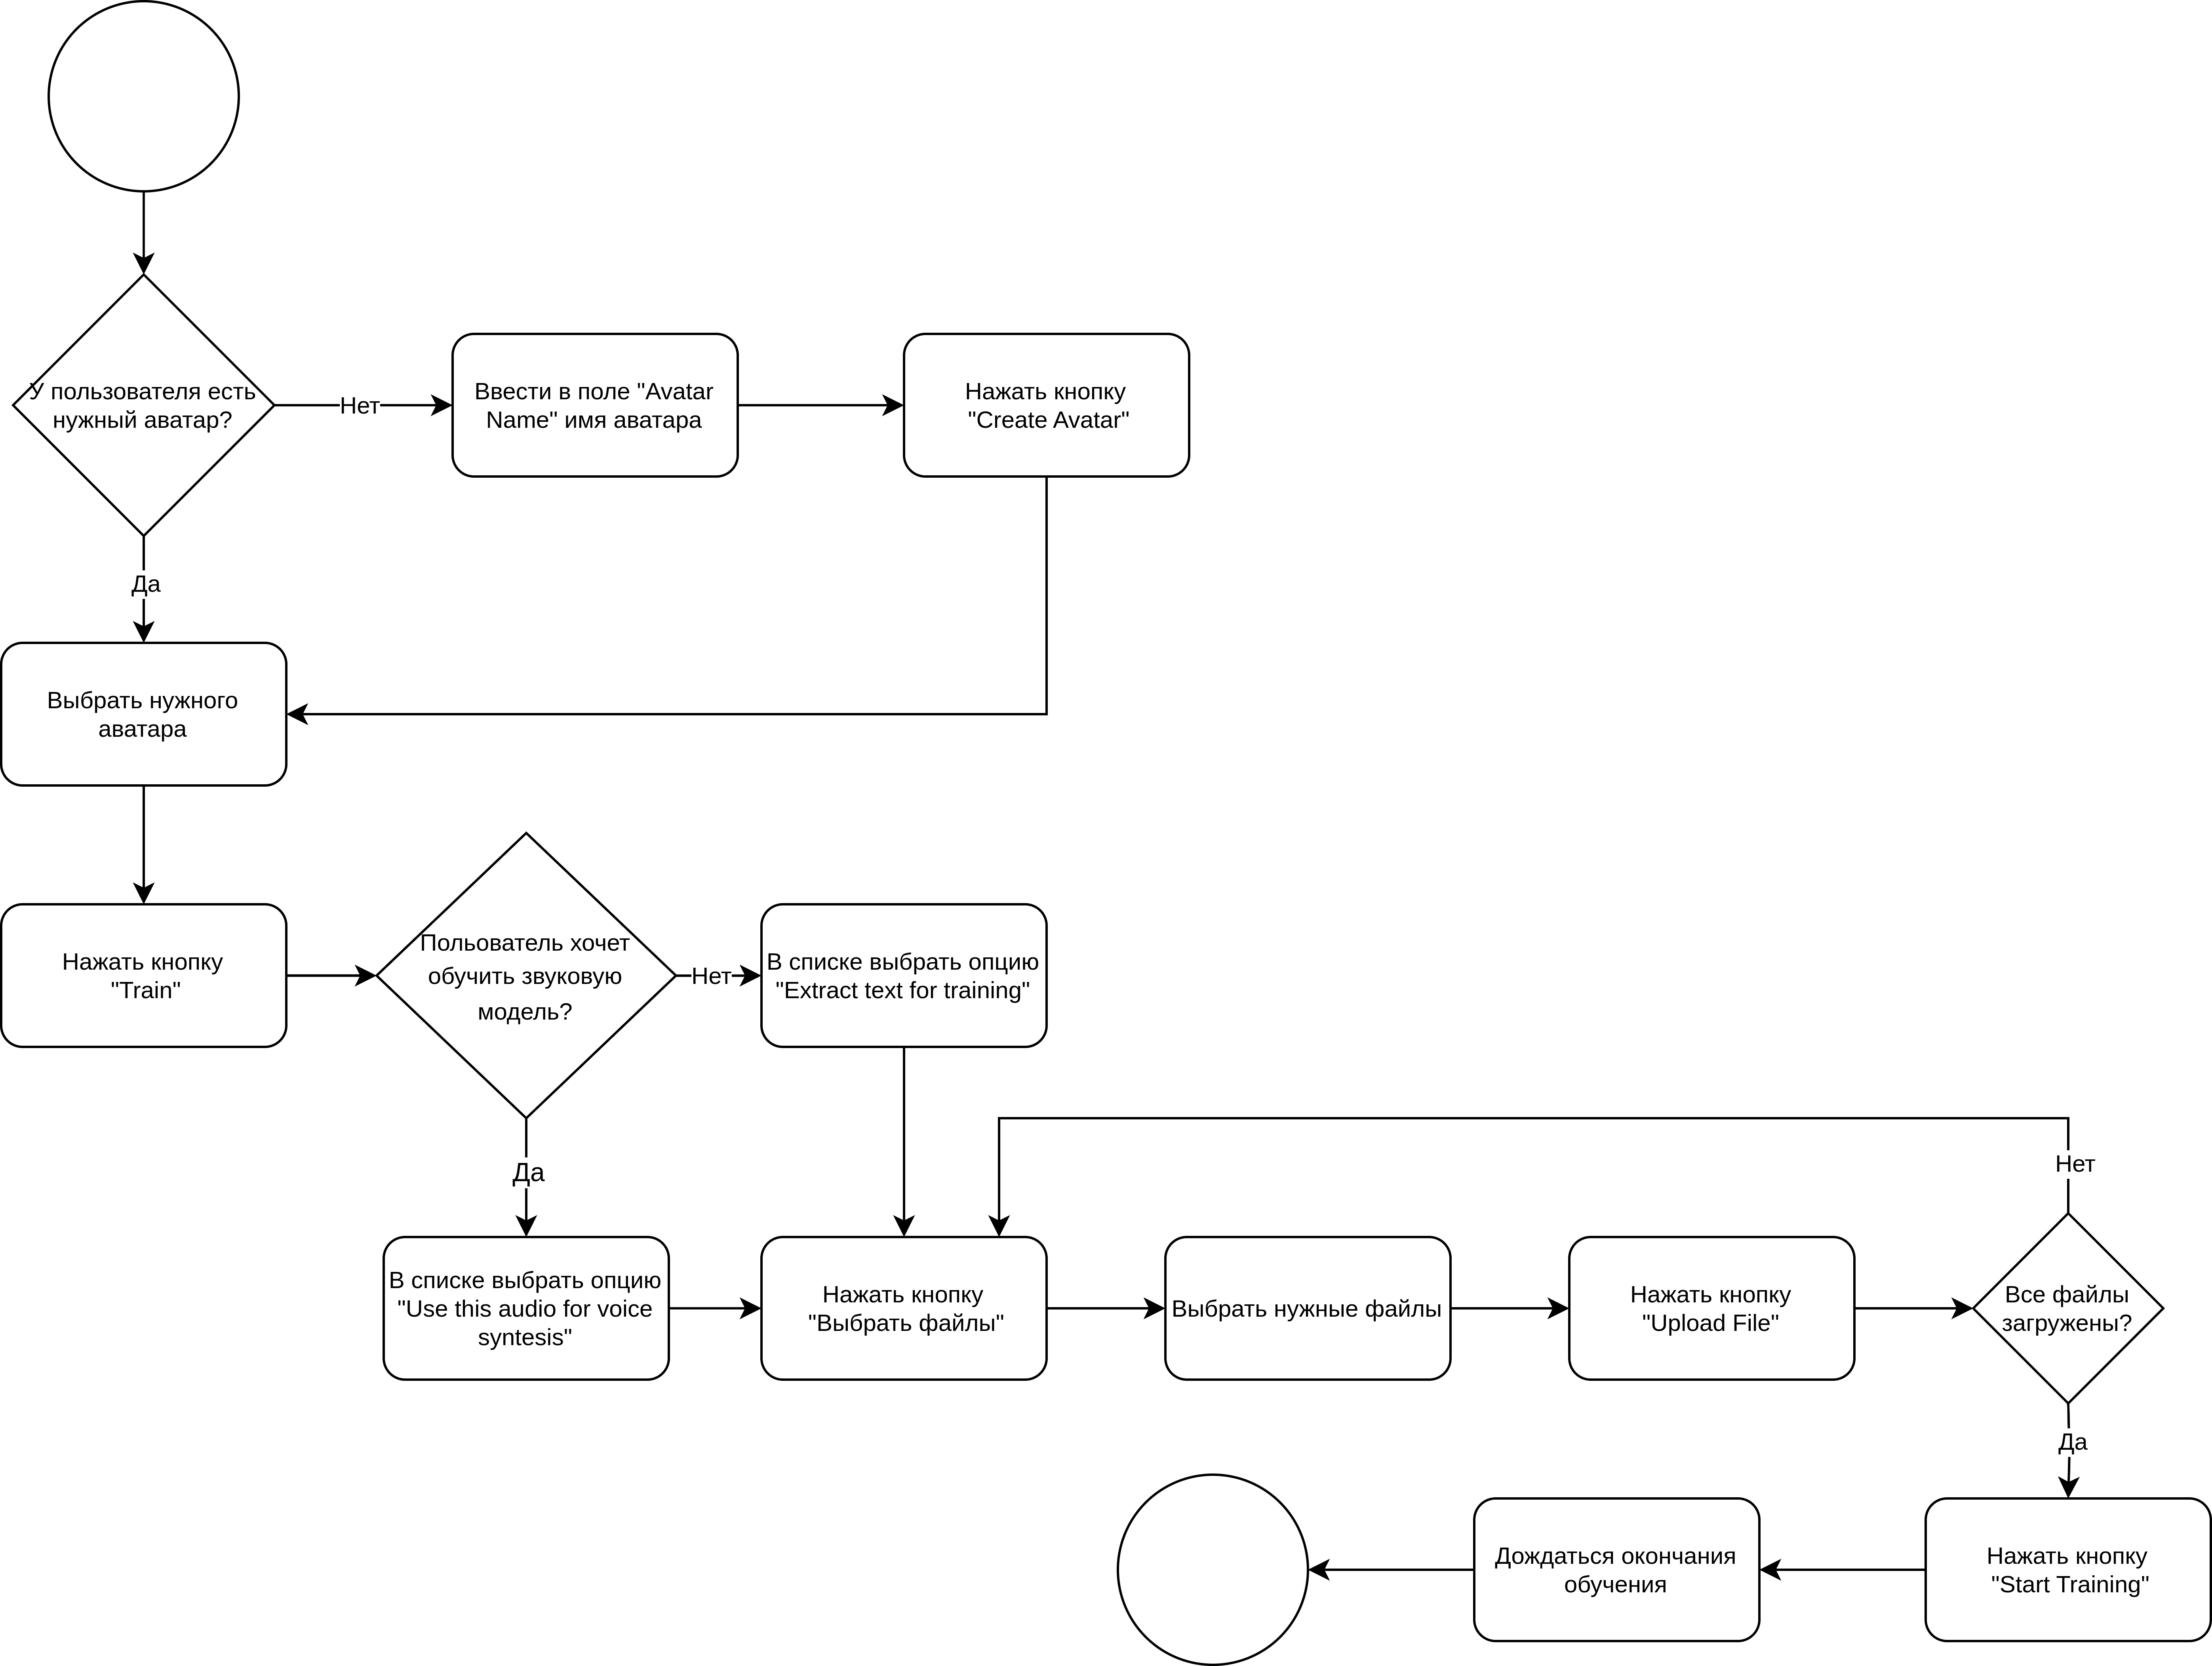
\includegraphics[width=1.0\linewidth]{images/UF-train-avatar.png}
    \caption{User flow диаграмма процесса обучения (пользователь уже выполнил вход)}
    \label{fig:uf-train}
\end{figure}

\subsection{Процедура взаимодействия с аватаром}
Аналогично процессу обучения на диаграмме процесса генерации (рис. \ref{fig:uml-inference}) отражены основные сообщения и события, через которые проходит система для предоставления пользователю сгенерированного текстового ответа и его озвучки на запрос. Аналогично представлен путь, через который проходит пользователь для создания запроса и получения ответа на user flow диаграмме (рис. \ref{fig:uf-chat-with-avatar})

 \begin{figure}[h!]
     \centering
     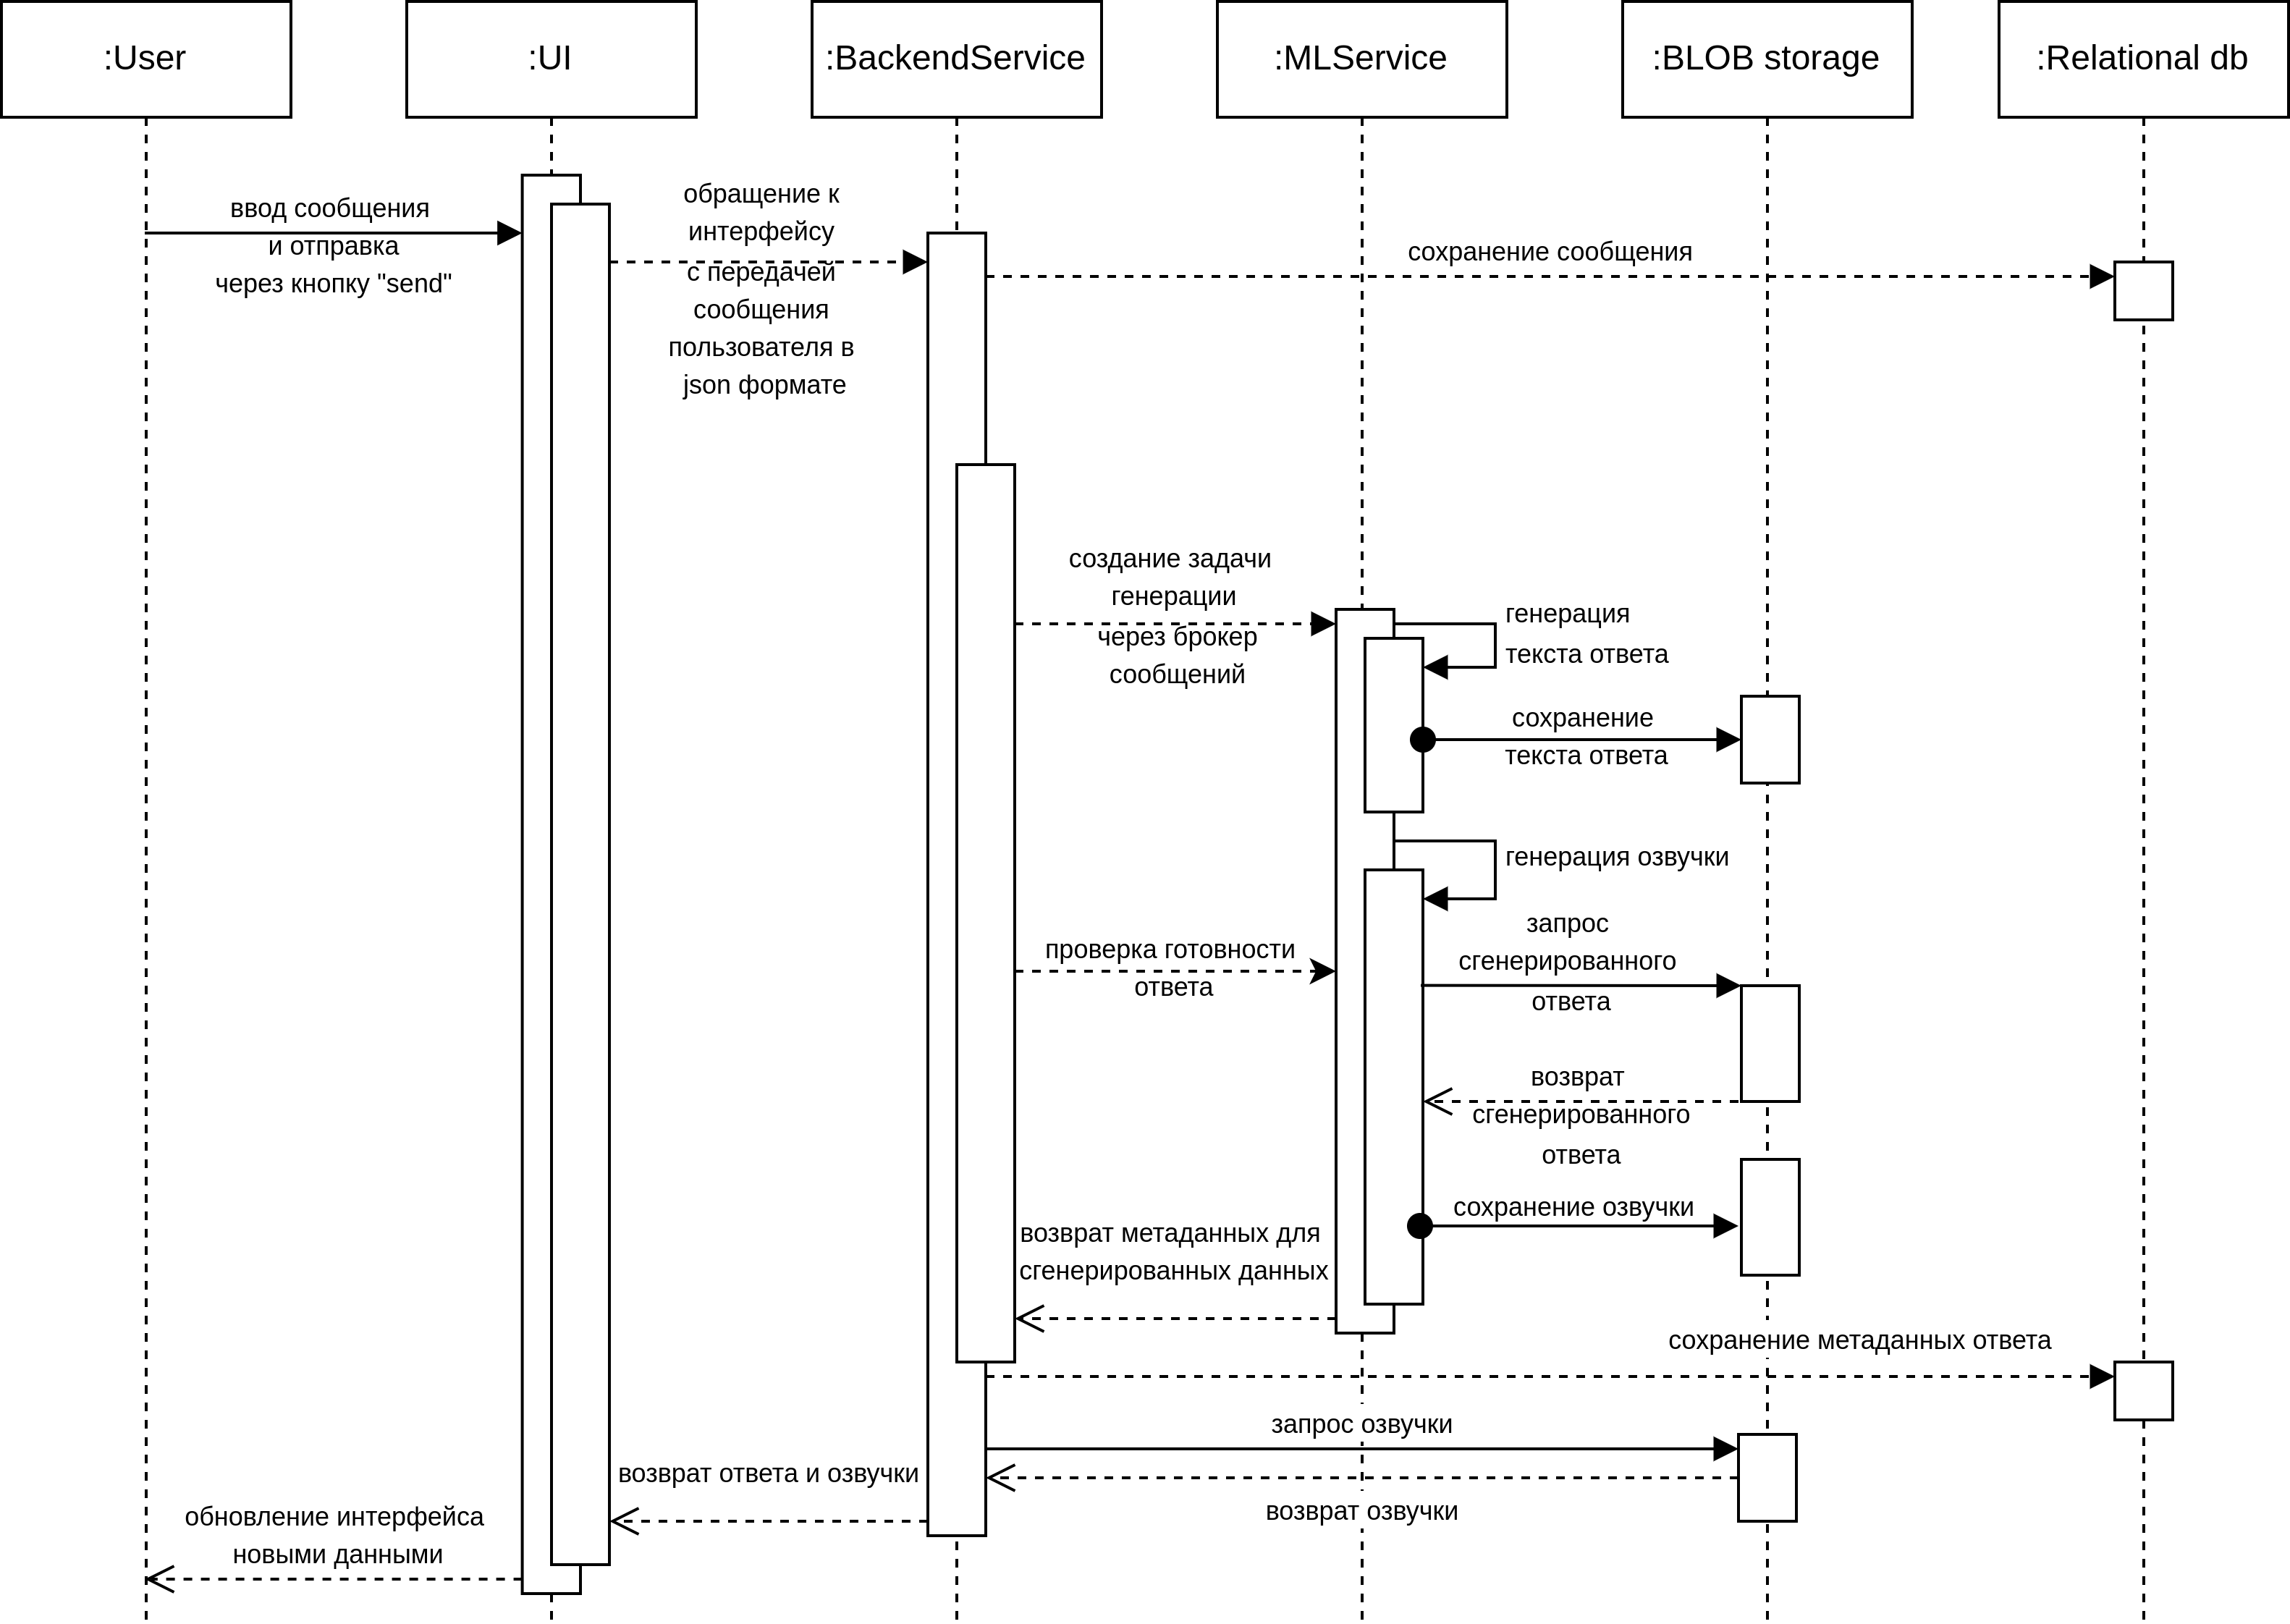
\includegraphics[width=1.0\linewidth]{images/uml-inference-rus.png}
     \caption{UML-диаграмма процесса генерации}
     \label{fig:uml-inference}
 \end{figure}
 \begin{figure}[h!]
    \centering
    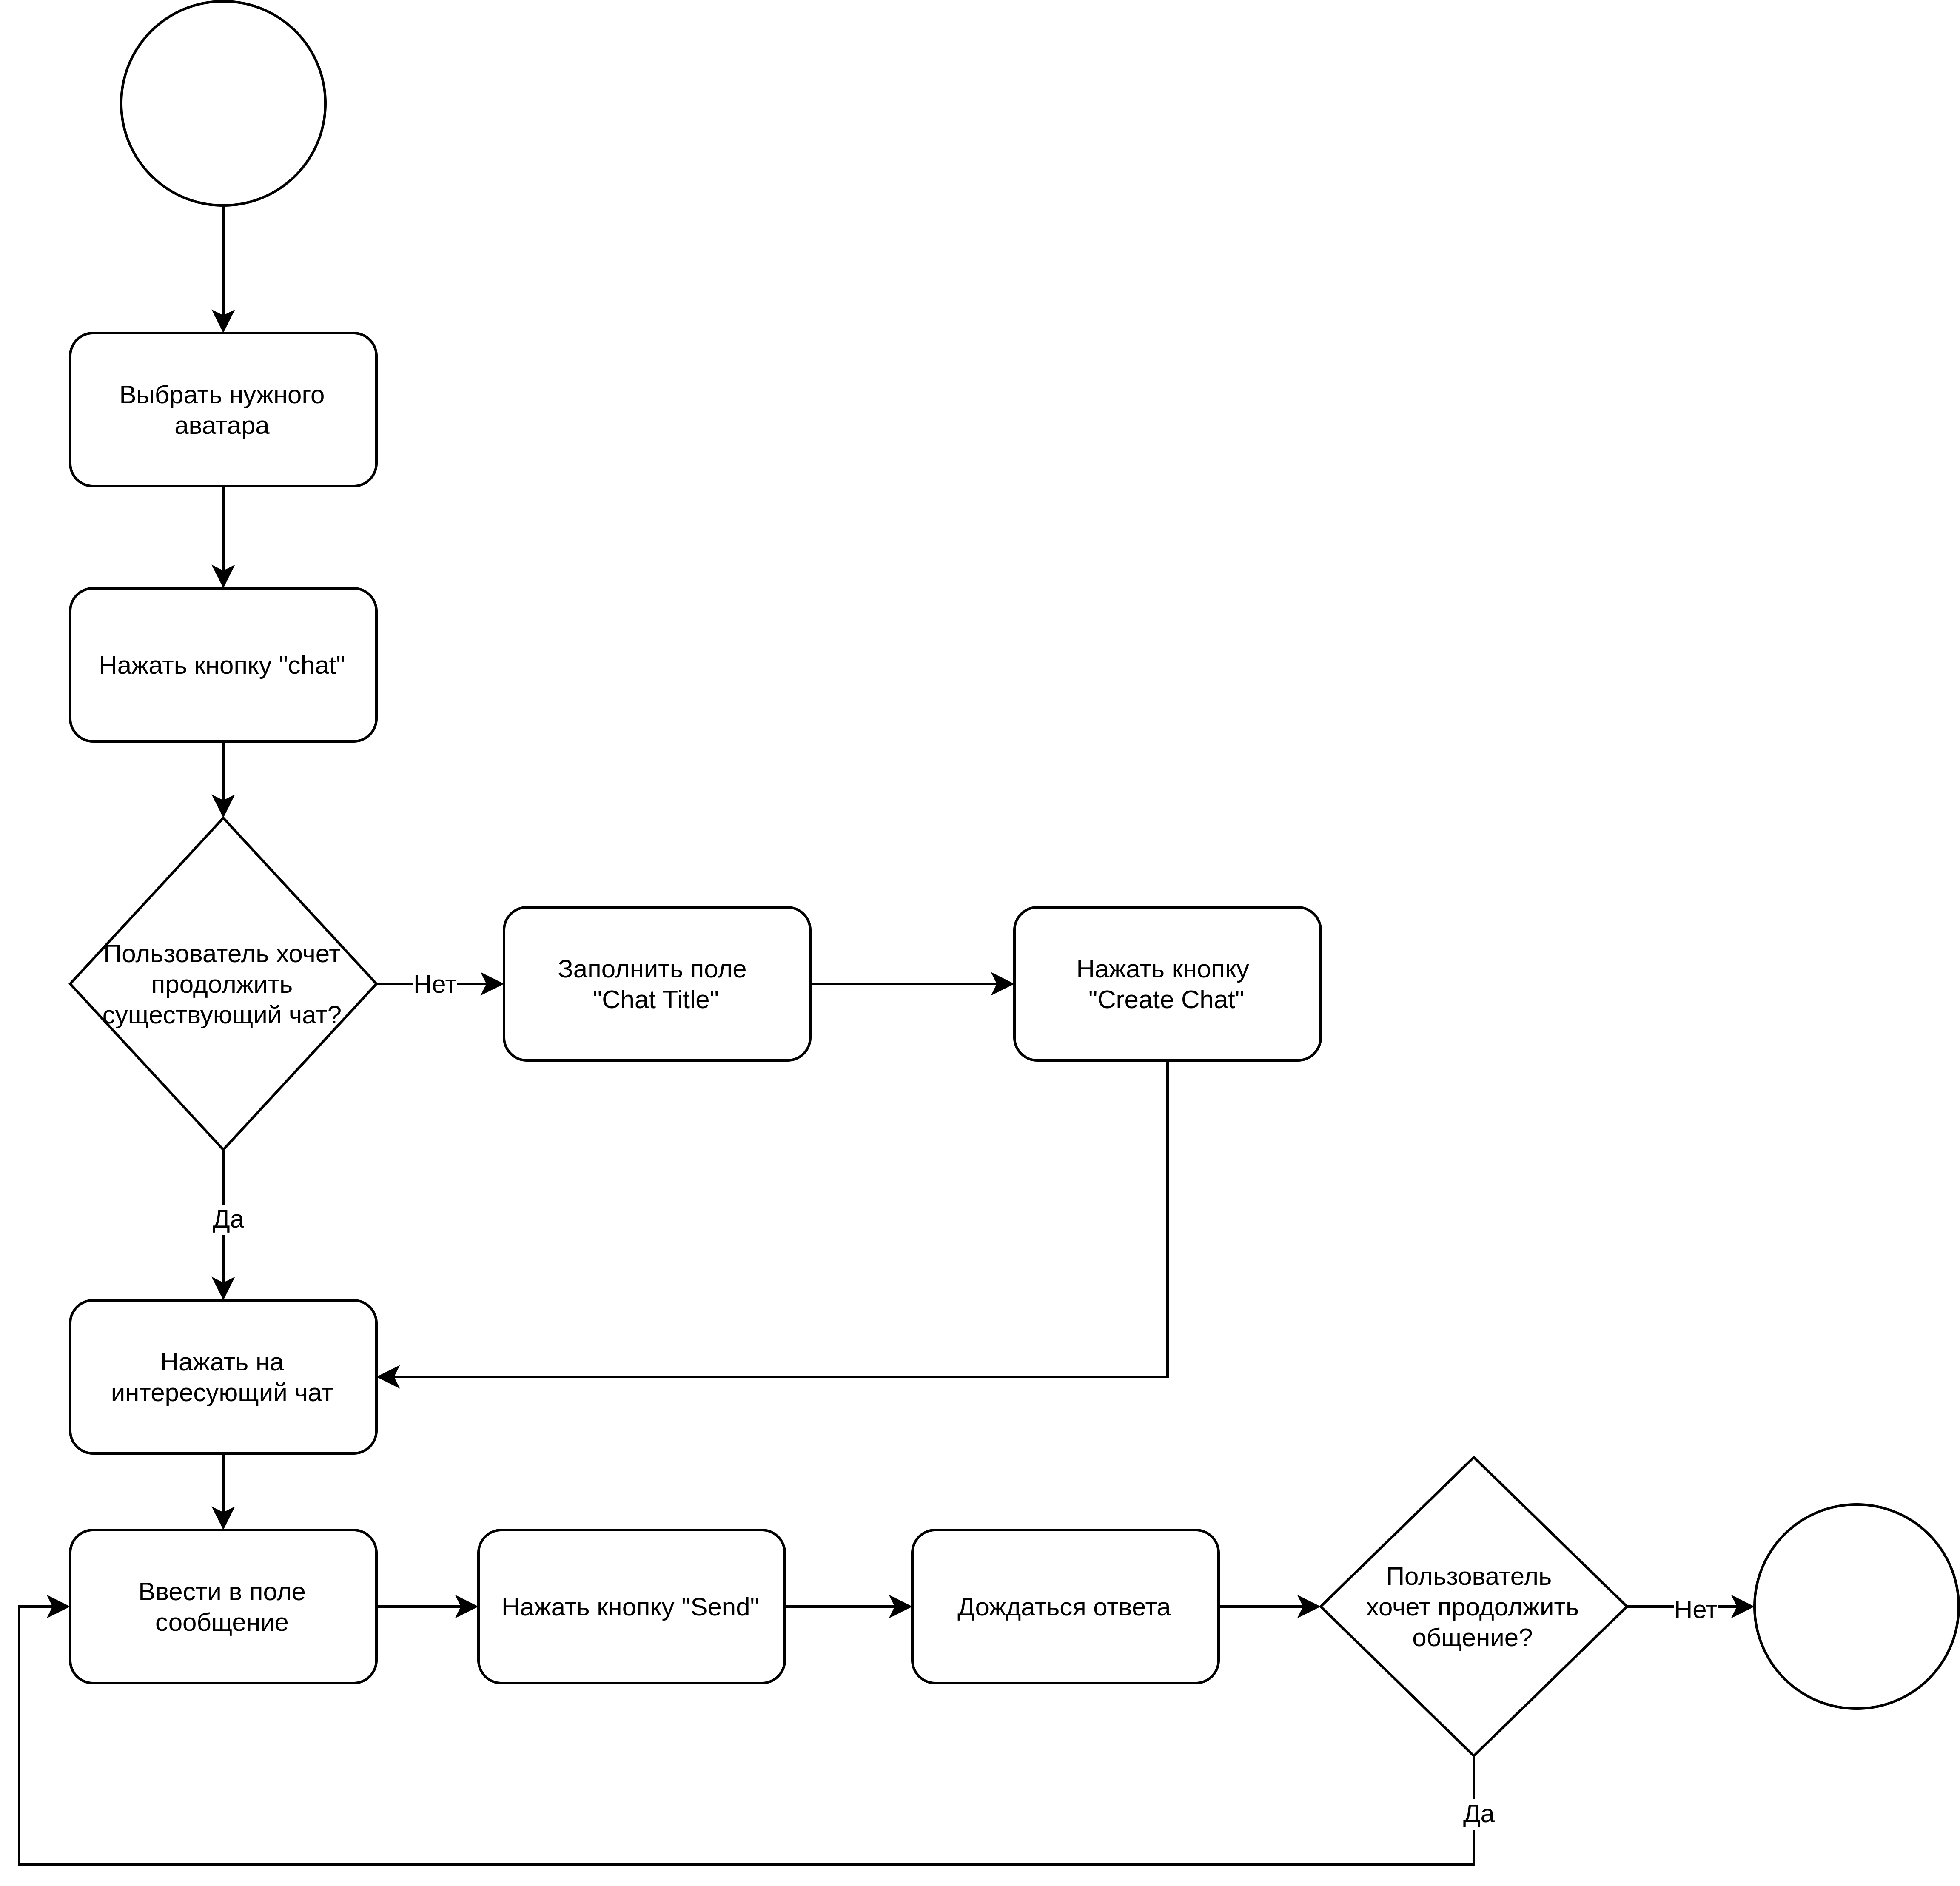
\includegraphics[width=1.0\linewidth]{images/UF-chat-with-avatar.png}
    \caption{User flow диаграмма процесса взаимодействия с аватаром (пользователь уже выполнил вход)}
    \label{fig:uf-chat-with-avatar}
\end{figure}

%FIX ME PLEASE
\begin{figure}
    \centering
    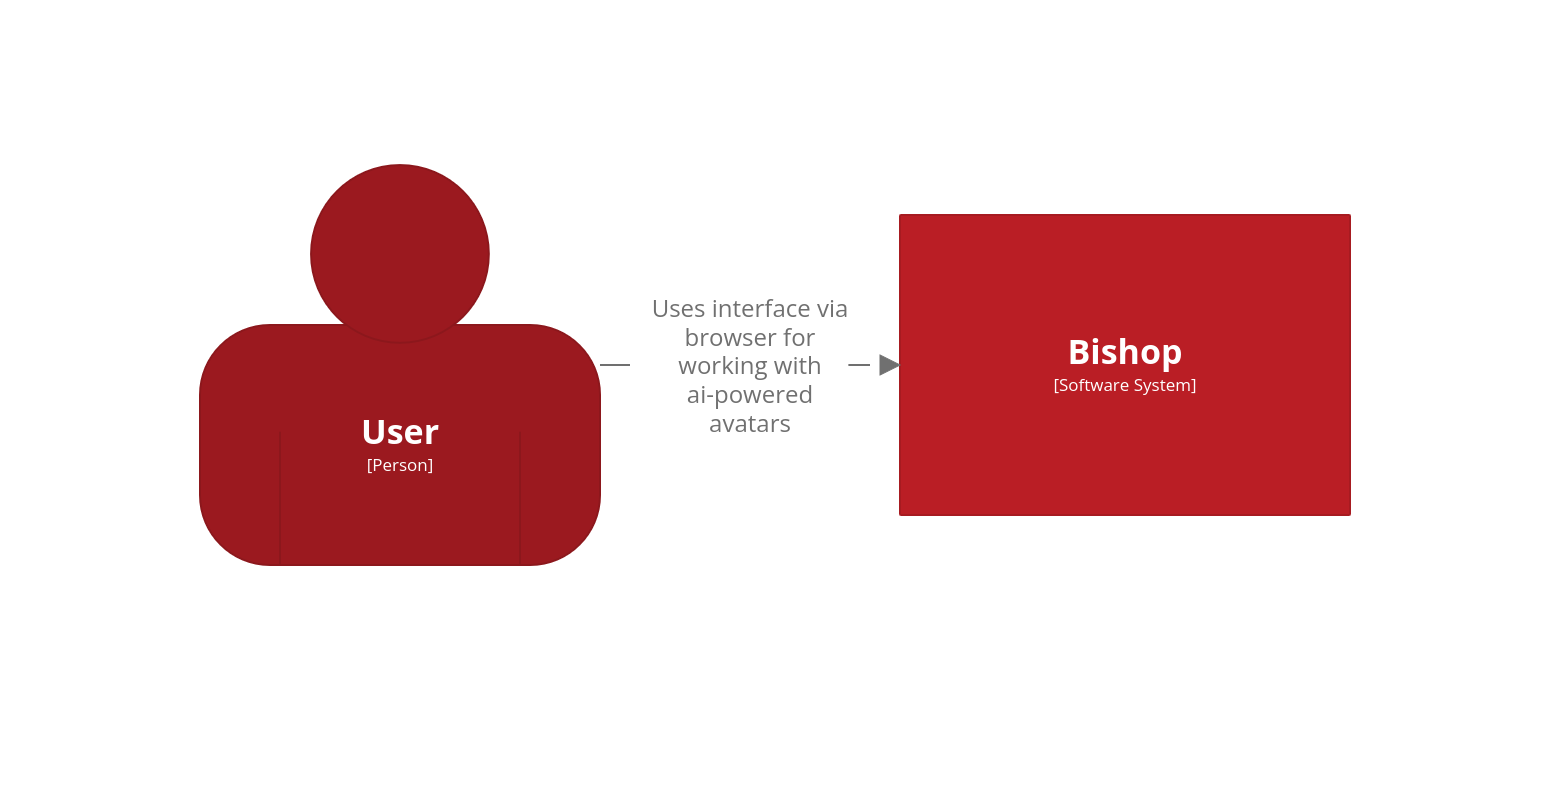
\includegraphics[width=1.0\linewidth]{images/c4-general.png}
    \caption{C4 диаграмма для сервиса <<Bishop>>}
    \label{fig:c4-bishop-1}
\end{figure}

\begin{figure}
    \centering
    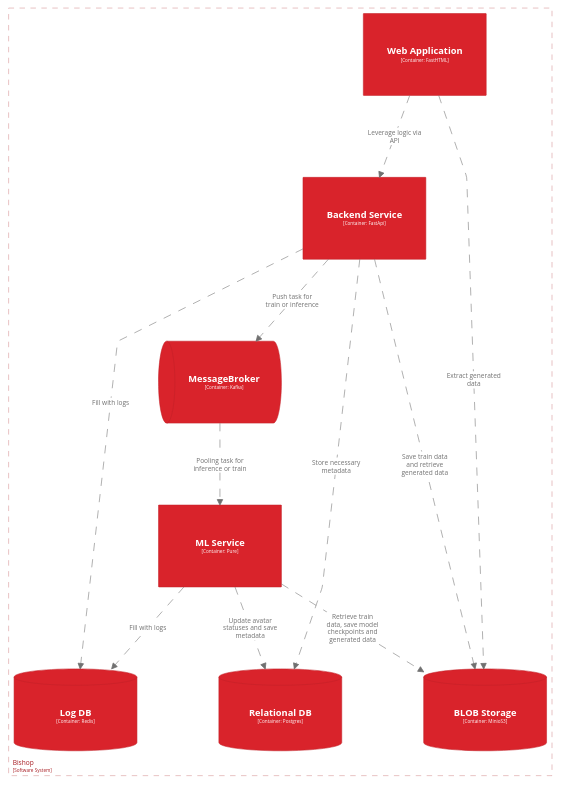
\includegraphics[width=1.0\linewidth]{images/c4-bishop.png}
    \caption{C4 диаграмма для сервиса <<Bishop>>}
    \label{fig:c4-bishop}
\end{figure}
